\documentclass[tikz,border=5mm,12pt]{standalone}
\usepackage{xcolor}
\usetikzlibrary{arrows.meta}

\newcommand\bw{12.5mm}
\newcommand\bh{10mm}
\newcommand\bbx{6mm}
\newcommand\bby{4mm}
\newcommand\arrw{18mm}
\newcommand\arrh{8mm}

\begin{document}
  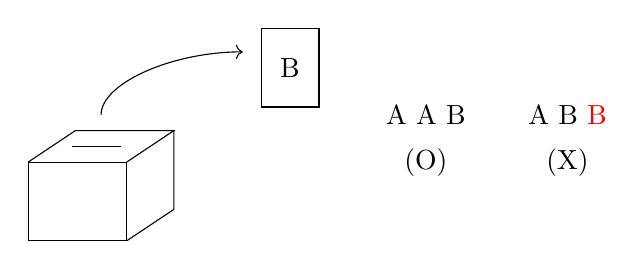
\begin{tikzpicture}
    \begin{scope}
      \draw (0,0) -- ++(\bw,0) -- ++(0,\bh) -- ++(-\bw,0) -- cycle;
      \draw (\bw,0) -- ++(\bbx,\bby) -- ++(0,\bh);
      \draw (\bw,\bh) -- ++(\bbx,\bby) -- ++(-\bw,0) -- ++(-\bbx,-\bby);
      \draw (0.3*\bw+0.3*\bbx,\bh+0.5*\bby) -- ++(0.5*\bw,0);

      \draw[->] (0.5*\bw+0.5*\bbx,\bh+\bby+2mm) .. controls +(up:0.5*\arrh) and +(left:0.5*\arrw) .. ++(\arrw,\arrh);

      \path (0.5*\bw+0.5*\bbx+\arrw+6mm,\bh+\bby+\arrh) coordinate (p);

      \node[text centered,text width=5mm,minimum height=10mm,draw] at (p) {B};
    \end{scope}

    \begin{scope}[xshift=\bw+\bbx+\arrw+14mm,yshift=16mm]
      \node at (0,0) {A A B};
      \node at (0,-6mm) {(O)};

      \node at (18mm,0) {A B \textcolor{red}{B}};
      \node at (18mm,-6mm) {(X)};
    \end{scope}
  \end{tikzpicture}
\end{document}
